\documentclass[]{article}
\usepackage{amsmath}
\usepackage{graphicx}

\begin{document}


OK, if I compare MSE for $\beta$ directly, it indeed cause the problem. Take 1/0 (\textbf{code 1}) vs. 1/-1 (\textbf{code 2}) as an example. Let the intercept and coefficient for categorical variable be $\beta_0$ and $\beta_c$ for \textbf{code 1}, while  $\beta'_0$ and $\beta'_c$ for \textbf{code 2}. Then $\beta'_0 = \beta_0 + \beta_c/2$ and $\beta'_c = \beta_c/2$. So the variance of $\boldsymbol{\breve{\beta}} - \hat{\boldsymbol{\beta}}_{MLE}$ for \textbf{code 2} will be smaller than \textbf{code 1}, because $\beta'_c = \beta_c/2$. This will lead to a lower MSE for \textbf{code 2}.

To fix that, I now compare the MSE for linear predictor, i.e. define MSE as $S^{-1}\sum_{s=1}^{S}\frac{||\boldsymbol{X}\breve{\boldsymbol{\beta}}^{(s)} - \boldsymbol{X}\hat{\boldsymbol{\beta}}_{MLE}||^2}{n - p}$

Now, To make the results more significant, I only include 1 continuous variable with one categorical variable with 2 levels. 

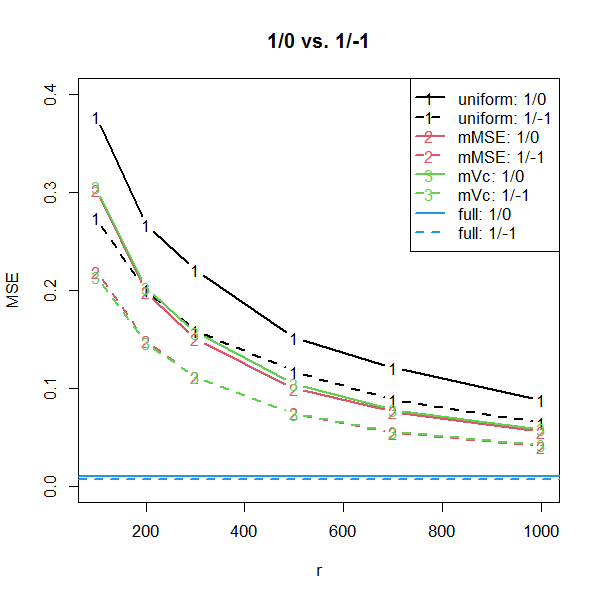
\includegraphics[width = .8\textwidth]{plot_2levels.png}

It seems that coding baseline as (-1, -1) is worse than coding as (0, 0). As we can imagine, coding the baseline with less absolute values will make things better. Here I use the same data, but code the baseline as (2, 2):

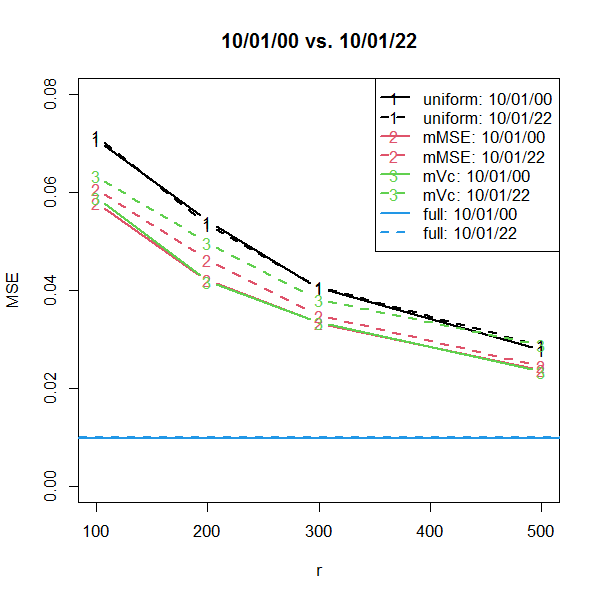
\includegraphics[width = .8\textwidth]{plot_2levels_2.png}

Now, it looks much worse, especially for L-optimization. (A-optimization is somewhat more robust to different coding, because of $\boldsymbol{M}_{X}^{-1}$ term)

Based on this observation, I may suggest to code the variable with least total absolute values (or the smallest Frobenius norm for dummy variable matrix (?)), without loss of interpretation. In other words, we should include as much 0 as possible.


Potential explanation:

Still consider L-optimization:
\begin{equation*}
	\pi_{i}^{mVc} = \frac{|y_i-p_i(\hat{\beta}_{MLE})||\boldsymbol{x}_i||}{\sum_{j=1}^{n}|y_i-p_i(\hat{\beta}_{MLE})||\boldsymbol{x}_i||}
\end{equation*}
If the dummy variable is coded as large absolute values, it will let the dummy variable guide the SSP, and this will cause bias?

	
\end{document}


